\documentclass{article}

\usepackage{graphicx}
\usepackage{hyperref}
\usepackage{amssymb}

\title{Yelp and Crime}  % TODO
\author{Kenneth Lin, Sid Naik, Tom McCormick}
\date{\today}

\providecommand{\e}[1]{\ensuremath{\times 10^{#1}}}

\renewcommand{\labelitemi}{\checkmark}

\begin{document}
\maketitle

\section{Problem Statement and Background}

For our CS 194 final project, we decided to investigate the potential
relationship between the City of San Francisco public safety data set and
the data set provided by the Yelp API. With the recent civil unrest both
inside and outside of the United States, and more recently, right here in
Berkeley, we thought that it would be interesting to look into the factors
that promote crime. One of our team members (Kenneth Lin) had also been
robbed recently, so the problem is one that is dear to our hearts. Perhaps
the most well-known correlation with crime rate is the income level of a
neighborhood -- the lower the income level, the higher the crime rate
\cite[p.93-94]{levitt-the-changing-relationship}. However, we wanted to
show something more interesting. In particular, Yelp restaurants, in our
experience, often reflect the wealth and well-being of its surrounding
neighborhood -- the presence of many highly rated restaurants, we believed,
reflect the optimism in the economy of a neighborhood, as well as the
wealth and ``goodness'' of that neighborhood. Therefore, we had conjectured
that crime would negatively impact restaurant ratings, or that low
restaurant ratings would be correlated with areas of high crime. We worked
to show this throughout our project.

% At first, we explored each data set individually to discover general
% patterns in the data set. After that, we delved into our main problem. We
% are interested in the relationship (if any) between the quality of
% restaurants and the frequency and severity of crime. In particular, we
% wanted to know

In particular, we wanted to know

\begin{itemize}
\item the effect of crime on restaurant ratings (or vice versa)
\item the distribution of crime vs. the distribution of ratings
\end{itemize}

We had also wanted to predict crime density / severity using restaurant
ratings or vice versa, but along the way we ran into issues of determining
or implying causation in any of the methods we used. By using one to
predict the other and trying to draw useful conclusions from this, we run
the risk of assuming causation without definitive proof. There are many
other problems that may arise as a result of this, which will be discussed
in the \textbf{\nameref{sec:lessons-learned}} section.

\subsection{City of San Francisco Public Safety Data Set}

The City of San Francisco public safety data set is a record, written by
the San Francisco Police Department, of incoming incident reports, either
via phone call, in person, or otherwise. These incidents, reported via the
SFPD CABLE crime incident reporting system, cover the span of more than 11
years, from 1/1/2003 to present. Incidents are recorded when a police
report is filled out during or after a crime incident. Crimes range from
aggravated assault to vandalism to death reports.

A sample of records in the data set looks like the following:

\begin{center}
  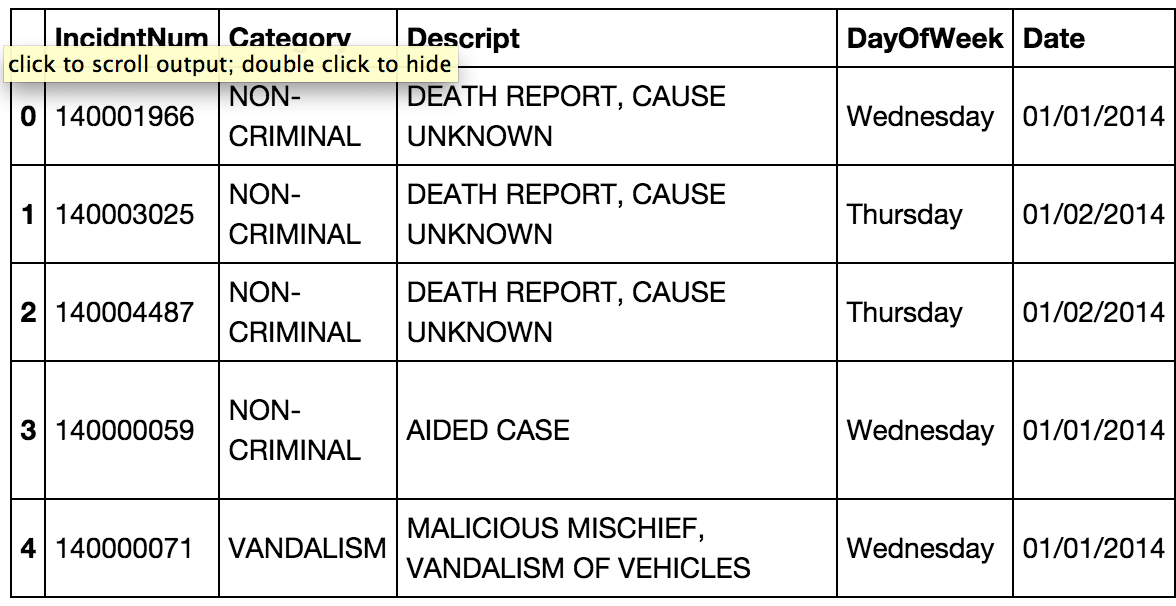
\includegraphics[scale=0.5]{sf_city_sample_1.png} \\
  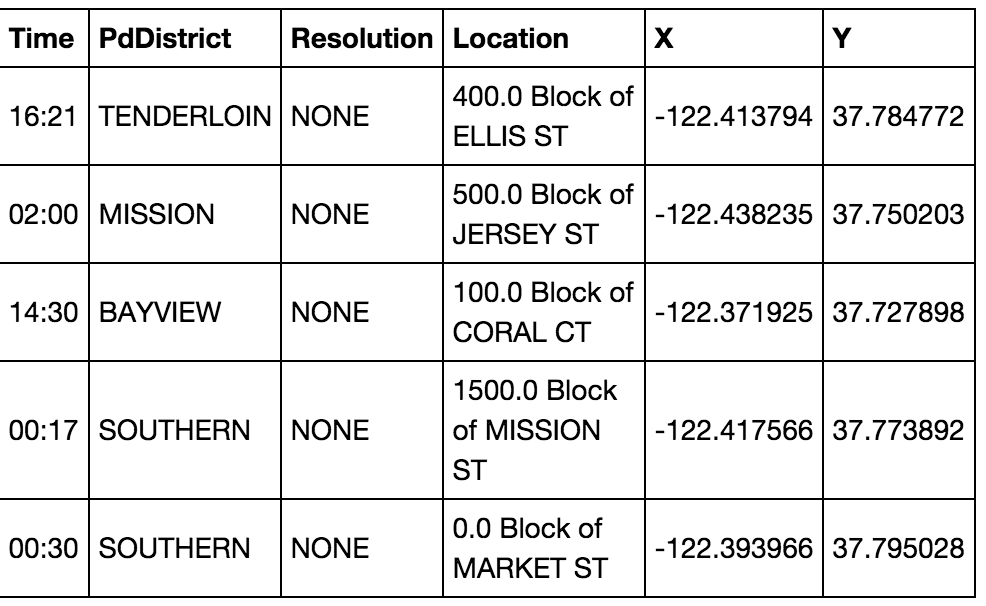
\includegraphics[scale=0.5]{sf_city_sample_2.png} \\
  Figure 1: Sample of San Francisco crime data set
\end{center}

The majority of the fields are self-explanatory. However, there are a few
things to note:
\begin{enumerate}
\item Category and descript are both categories, but category is more
  general. There are only 36 different ``Categories'' while there are 499
  different ``Descript''s in the year of 2014.
\item Resolution, though none are shown in the sample above, denote whether
  any action was taken and what that action was.
\item X denotes longitude, while Y denote latitude.
\end{enumerate}

A more detailed analysis is in the attached \texttt{analysis.ipynb}.

\subsection{Yelp Data Set}

Yelp.com is a platform which publishes crowd-sourced reviews about local
businesses. On Yelp, customers who have used the services of local
businesses may write reviews of these businesses and provide ratings of
their satisfaction. Reviewers may select from between 1 to 5 stars for each
review they make, and a business's average rating is the average of the
ratings of each of the reviews it has received. Yelp supplies a platform
for all kinds of local businesses ranging from restaurants to barbers to
museums; however, for the purpose of our research, we will look primarily
at restaurants as they are a very large majority of the reviews on Yelp.

There are two primary ways to access the data on Yelp. First, we can
utilize the search / business API
(\url{http://www.yelp.com/developers/documentation}). The API provides a
way to search for local businesses matching a particular key term
(``restaurants'', for example) near a geographical location, and get all
the rating / review information about that restaurant. The API further
allows us to narrow the search to only the geographically closest
restaurants (not ranked by rating). This gives us a way to link the
geographical location of crime incidents to the types of restaurants near
that incident.

The other way of accessing Yelp data is through the academic data set
(\url{https://www.yelp.com/academic_dataset}). The Yelp academic data set
provides all the data and associated reviews of the 250 closest businesses
to each of 30 universities, including UC Berkeley. Although not a random
sample of all businesses on Yelp, the academic data set provides a much
better estimate of all businesses in the Yelp data set population. For the
purposes of the analysis, we will assume for now that this data set is
a perfect sample of the entire Yelp data set, and that its average is
indicative of the Yelp-wide average. Issues with this assumption will be
addressed in the \textbf{\nameref{sec:lessons-learned}} section.

\section{Methods}

\subsection{Data Fetching}

The bulk of our work was done in trying to get data from Yelp. As
mentioned, there were two main ways that Yelp provides to access data, and
those are the API and the academic data set.

To access the Yelp API, Yelp provided sample Python code
(\url{https://github.com/Yelp/yelp-api/tree/master/v2/python}). However, as
we found out, the sample code was buggy -- not only did the code fail on
certain calls, it even failed on the default call when the search term was
``dinner'' and the location was ``San Francisco, CA''. We contacted Yelp
API support about this issue, but it seemed that the API wasn't
well-maintained, and Yelp engineers didn't have time to update or fix the
sample code. Therefore, we decided to fix the bug ourselves.

After much investigation, we figured out that whereas Python's
\texttt{urllib} library encoded spaces into ``+'' characters, Yelp's
server-side authentication expected the OAuth-signed URLs to use ``\%20''
as the proper encoding for space. In this context (the query arguments in a
URL), both should be valid, but Yelp's authenticator only expected the
latter. After figuring this out, we let the Yelp engineers know of the bug,
and were able to begin building a temporary work-around to fetch our data.

We also encountered other problems in data fetching. In addition to the
bugs in the API, there were rate limiting and quantity limiting issues as
well. In particular, we could only access 20 results at a time, and a
maximum of 40 total results for searches that sorted the results by only
distance or rating. With searches not purely by distance or rating, Yelp
enforced its own ranking to its results. Results further down the results
page became so varied that they no longer matched the keyword (for example,
Yep may provide a gym even though ``food'' was specified simply because the
gym was much closer than any other ``food'' locations). All of the above
limited the ways in which we could obtain and analyze Yelp data.

For us, the ideal way to get Yelp data would be to have a data set
containing data on every single restaurant in San Francisco. This would
have been the most ideal solution as
\begin{enumerate}
\item we could then \textit{compare} the properties of restaurants near
  crimes to the general population of restaurants in San Francisco
  properly. The way we do this instead is to use the academic data set, but
  that includes data from other cities
\item the data we had would be the \textit{entire population} of restaurants in San
  Francisco (that Yelp has in their database)
\item we could then easily compare any other location-based data (like
  population density) and determine any confounding factors in our
  statistical model. This wasn't discovered until after our t-test results.
\end{enumerate}

Further, we weren't able to get as much data as we needed (because of
Yelp's rate limiting). However, it was still possible to search for the
closest restaurants near any location specified by longitude and
latitude. As a result, we decided to search for the 20 closest restaurants
near each crime and look at the characteristics of this set of restaurants.

In the end, we were able to build a fault-tolerant work-around to Yelp's
broken authentication system. We queried Yelp's API for the 20 closest
restaurants near each crime in the City of San Francisco crime data set for
a total of 12,000 crimes (9704 unique incidents due to multiple criminal
offenses per incident). These results were stored in the MongoDB instance
that we installed on our EC2 server.

\subsection{Visualization}

% TODO
% TODO do yelp rating map

\subsection{Looking for Correlations}

Our primary purpose (initially) was to determine how crime affected
restaurant ratings. Specifically, given the limitations of the data we
could get from Yelp, we wanted to see whether Yelp restaurant ratings were
any different when they were near crime hotspots.

At this point, we could access two data sets -- the data set of
``near-crime'' restaurants, obtained through querying for restaurants near
crime incident locations via the Yelp API, and the Yelp academic data
set. Given this data, we had a few options to draw a correlation:
\begin{enumerate}
\item We could look at the ``average rating'' of a crime -- that is, we
  could take the average rating of the 20 closest restaurants to a crime
  incident and call that the average rating of restaurants near that
  crime. Then, we could compare that rating with the Yelp-wide average from
  the academic data set.
\item We could look at all the \textit{restaurants} near any of the crime
  incidents in the crime data set. Then, we can put these together as a set
  of ``near-crime'' restaurants, and look at the rating distribution of
  these compared to the academic data set.
\end{enumerate}
We had originally planned to execute option 1. However, as we realized from
exploring the crime data set, crime density is very different for different
areas of San Francisco. If we look at the average rating of each crime, it
is likely that the results would be very heavily weighted by the ratings of
restaurants in high crime density areas (ie. Market Street). Although our
very purpose was to show that high crime density areas were prone to
different kinds of Yelp ratings, we did not want to artificially induce
this by weighting the results by the crime density itself. Therefore, we
chose the second option. Surprisingly, we discovered that in the 9704
unique incidents we looked at and the 194080 restaurants near those
incidents, there were only a total of 658 unique restaurants. This implies
that the crimes were indeed very clustered, and that use of the ``average
rating of a crime'' method (option 1) would have resulted in significant
bias to restaurants near the clustered areas. This will be discussed more
in the \textbf{\nameref{sec:lessons-learned}} section.

To determine whether there were any significant differences between the two
data sets, we used a Student's t-test as our statistical hypothesis
test. In this case, the null hypothesis was that the two data sets, both of
Yelp ratings in San Francisco, have identical expected values (means). The
t-test results are more thoroughly discussed in the
\textbf{\nameref{sec:results}} section. Through the analysis, however, we
learned instead that restaurants near high-crime areas actually had higher
ratings than the Yelp-wide average.

However, as we learned through % TODO explain correlation != causation

\subsection{Accounting for Population Density}

As a result of our findings, we realized that causation != correlation.
% TODO more

-- tract difficulties, calculating tract centers

\subsection{Predicting Crimes}

% TODO more subsections

\section{Tools}

\begin{itemize}
\item pandas -- Pandas was our primary means of manipulating data sets. We
  used Pandas in our data fetching, data cleaning, and data analysis
  process.
\item MongoDB -- We installed MongoDB on the EC2 server and used it
  primarily for storing Yelp data. MongoDB was a great choice because the
  document-based nature of MongoDB was perfect for storing all the JSON
  documents we received from the Yelp API. In addition, we weren't sure
  what kind of data we needed to store when we first began fetching data,
  so using Mongo allowed us to easily keep all of the data in case we
  needed more than what we had thought.
\item pyMongo -- pyMongo was our choice Python interface to MongoDB.
\item numpy -- NumPy was used in conjunction with both Pandas and SciPy.
\item scipy -- We used SciPy mostly for its large library of statistical
  methods (t-tests, etc.).
\item D3.js -- We used D3 in conjunction with other frameworks when
  visualizing the data.
\item Google Maps API -- The Google Maps API provided a base for many of
  the location-based visualizations we needed to create. In addition, the
  Google Maps API also had a heatmap plugin, which we tried in addition to
  heatmap.js.
\item heatmap.js -- We primarily used heatmap.js for our heatmap
  visualizations.
\end{itemize}

\section{Results}
\label{sec:results}

A preliminary analysis of just the public safety data set is available in
the attached \texttt{analysis.pynb}. Below follows our results and
conclusions from looking at Yelp restaurant rating data near crime
hotspots.

\section{Putting it together}

The results of the t-test between the near-crime data set and subsets of
the academic data set are detailed in Table 1.

\begin{center}
  \begin{tabular}{ | l | c | c | c | c | }
    \hline
    Data set                       & Mean  & Variance & t-statistic* & p-value*    \\
    \hline
    Near-crime                     & 4.072 & 0.107    &              &             \\
    All businesses (all)           & 3.618 & 0.871    & -12.441      & 2.39\e{-35} \\
    All businesses (Berkeley)      & 3.629 & 0.701    & -12.390      & 3.43\e{-33} \\
    All businesses (Stanford)      & 3.696 & 0.716    & -8.310       & 4.34\e{-16} \\
    All businesses (Los Angeles)   & 3.571 & 0.976    & -12.542      & 1.66\e{-34} \\
    Restaurants only (all)         & 3.482 & 0.545    & -20.291      & 7.10\e{-89} \\
    Restaurants only (Berkeley)    & 3.413 & 0.382    & -20.490      & 9.34\e{-77} \\
    Restaurants only (Stanford)    & 3.307 & 0.270    & -14.367      & 3.30\e{-41} \\
    Restaurants only (Los Angeles) & 3.431 & 0.598    & -18.797      & 2.28\e{-68} \\
    \hline
  \end{tabular}

  Table 1: t-test results against ``near-crime'' data set
\end{center}
* against the ``near-crime'' data set

The ``all businesses'' data sets refer to all the businesses provided by
the academic data set, whereas the ``restaurants only'' data sets filtered
out only the businesses in the academic data set that had ``Food'' or
``Restaurants'' as one of the items in its category field.

From the p-values of each t-test it is clear that the null hypothesis can
be rejected, and that the ``near-crime'' data set does not have the same
average Yelp rating as the other data sets. The following two plots provide
a better picture of the actual distribution of each data set.

\begin{center}
  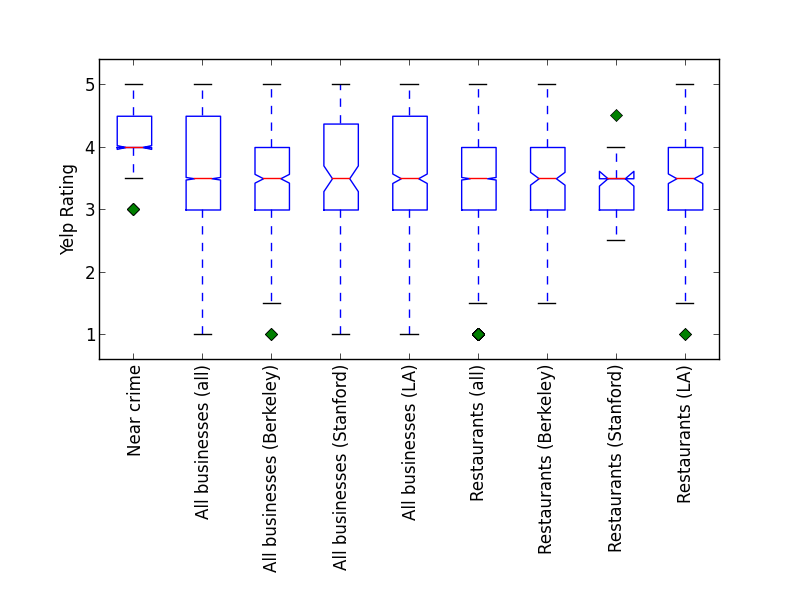
\includegraphics[scale=0.5]{boxplot.png} \\
  Figure 2: Box-and-whiskers plot of distribution of the ratings of
  different data sets

  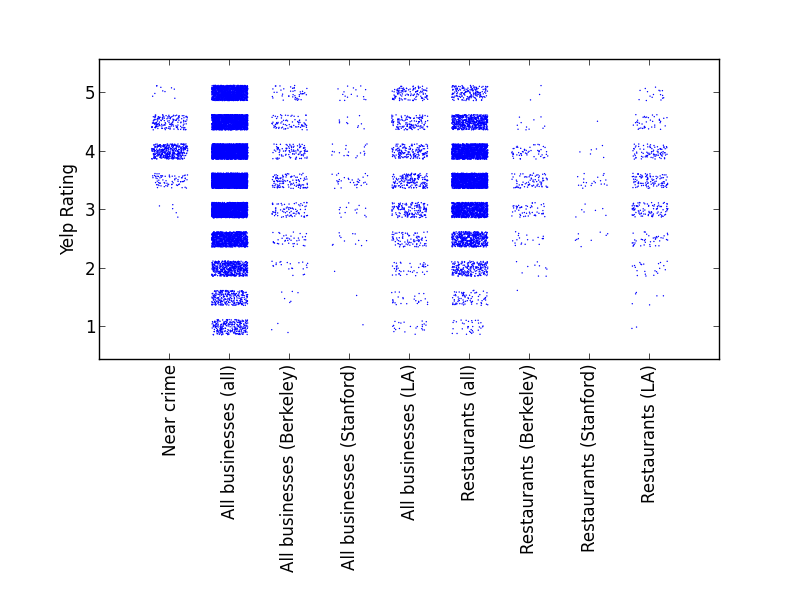
\includegraphics[scale=0.5]{scatter_plot.png} \\
  Figure 3: Scatter plot of distribution of the ratings of different data
  sets. Points plotted with certain randomness to show distribution of
  points.
\end{center}

However, the data indicates that our initial hypothesis was also wrong --
we found instead that the restaurants near crimes were actually
\textit{higher} rated than the general population of restaurants. To us,
this was extremely counterintuitive. Our original hypothesis was that crime
would negatively affect restaurant ratings. However, the data seems to show
that crime was instead positively correlated with ratings. As we were
looking for explanations, we also realized that the tests we have been
doing would not prove causation anyways. It's possible that crime
positively affects restaurant ratings, or that restaurant ratings increase
the crime rate, but it's also possible that both are correlated with a
third confounding factor. In particular, from the visualizations we created
earlier, it's very likely that population density would be a factor. Areas
near Market Street are known to be the most popular areas in San Francisco,
for work, shopping, and many other things. As we were not familiar with
these statistical notions when we formulated our problem statement, we had
not thought of problems like these when we started.

Due to the limitations of the Yelp API, we could not get Yelp data with an
even distribution across all of San Francisco. Given what we had, we wanted
to compare the population density of the areas of near-crime restaurants to
the population density of the restaurants in the other sets. However,
because our academic data set had restaurants all across the United States
where we didn't have ready access to population density data, it was
impossible to calculate population density for these areas. Further,
population varies more by city than areas within the city, so variations in
those restaurants are not telling at all.

The best alternative was to instead compare the population density of the
areas of near-crime restaurants to the total population density of San
Francisco. Although the results of this test would not be directly related
to the test performed above, it would provide exploratory insight into the
reason behind why our hypothesis was wrong.

% TODO why do we go to population density

% TODO where to put correlation vs causation

-- distribution
-- ratings

-- CONCLUSIONS??!?

-- map visualization problems
---- yelp data biased to near crime
---- not enough data on all of san francisco to create proper viz

-- condition tests in certain neighborhoods

\section{Lessons Learned}
\label{sec:lessons-learned}

-- Yelp API shit; no one uses
-- data cleaning hard
-- causation and correlation
-- tract difficulties
-- clear problem statement
----> not our fault, more because we didn't have experience with data
science projects and no proper guidance
-- problems with the data (not sure where it's from)
-- don't draw conclusions before the results are out
-- note about Yelp data not having ``price'' characteristic
-- academic data set biased
-- keyword match problems

-- IMPORTANT: COULD NOT GET CITY WIDE DATASET EASILY, so resort to strange
/ weird separate tests
----> no such thing as ``city-wide average''
----> can't predict for rest of SF yelp data set because can't access
----> should have gotten Yelp rating per tract / area so can compare with
crime density and population density per tract

-- must stress, given the limitations we did pretty well

\bibliographystyle{IEEEtran}
\bibliography{writeup-bibliography}

\end{document}
